
\section{Introduction}

So far, we have mostly focused on `scalar' active matter whose continuous description
is generally expressed in terms of a scalar density field.
In this chapter, on the contrary, we will address cases where active systems present large scale orientational order.
The goal of these lectures is to present a minimalist approach to this problem, which consists of building simple models 
including relevant physical ingredients so as to capture physical features common to a broad variety of active matter systems.
We will start by adopting a microscopic point of view, i.e. by constructing a particle model for collective motion.
Then, as we will be interested in collective effects involving many individuals, 
we will coarse grain our model using kinetic theory in order to obtain its hydrodynamic description
which will allow us to theoretically characterize the large scale physics at play.

\section{A minimal approach to collective motion} 

Collective motion can be described as the ability of some self propelled agents to move coherently at the level of many individuals without the need of a leader or external influence.
Such definition encompasses various examples found in nature, 
most obvious are human crowds, bird flocks, or insect swarms.
At the micron scale one can moreover mention bacterial colonies, or cellular migration which is involved in various biological phenomena such as morphogenesis, wound healing, or cancer development.
Cells are actually put into motion thanks to an elaborate machinery involving various types of molecular motors, so that collective motion is also found at sub-cellular scales (cf~\autoref{chap_intro}).

A natural question for a physicist is then whether all the above systems, even though their size spans many orders of magnitude, share common {\it universal} properties which could be captured by a unified theoretical framework.
To answer this question, we will adopt a minimalist approach that will discard the details of each system, but only include the physically relevant ingredients necessary for collective motion to arise.

\paragraph*{How physicists see birds}
In the past thirty years, flocks of birds became one of the paradigmatic examples of biological active matter. A combination of tracking experimental data and theoretical approaches based on statistical physics allowed to unveil and quantify many properties of their collective behavior. 
When moving along a fixed direction, 
the large cohesive structures formed by birds can be seen as breaking the global symmetry of rotation.
In analogy with liquid crystal physics, the velocities $\{\bm v_i\}_{i = 1,...N}$ of birds 
thus exhibit a certain amount of order,
which can be quantified computing the average polarization
\begin{equation}
\Pi(t) = \left | \frac{1}{N} \sum_{i}^N \frac{\bm v_i(t)}{|\bm v_i(t)|} \right |
\end{equation}
which is $1$ for a perfectly aligned system, and it is $0$ for a disordered one.
The average value for flocks is around $\langle \Pi \rangle \sim 0.96$, reflecting a high degree of polar order. However, this feature is not enough to ensure a self-organized collective behavior of the group. Birds move without a leader, interact with only a few neighbors, but their motion is correlated on length scales much larger than the typical inter-element distance. This has been understood looking at the individual velocity fluctuation around the mean velocity of the group,
$$
\delta \bm v_i (t) = \bm v_i(t) - \frac{1}{N} \sum_k \bm v_k(t)
$$
and at its correlation function,
\begin{equation}
 C(r) = \frac{1}{C_0} \left\langle \frac{\sum_{ij} \delta \bm v_i(t) \cdot \delta \bm v_j(t) \delta(r-r_{ij}(t))}{\sum_{ij} \delta(r-r_{ij}(t))} \right\rangle_t
\end{equation}
that measures how much the fluctuation in the moving direction of bird $i$ influences that of bird $j$, when they are separated by a distance $r_{ij}$. $C(r)$ is a static quantity, thus averaged over all the trajectories. 
\autoref{scalefree} shows this function obtained from experimental data from real flocks: the correlation is positive for short distances, then it decays until crossing the zero at a point $\ell_c$, and finally it becomes negative. This last feature is due to the definition of velocity fluctuation, but this trend highlights that there are only two large correlated domains in the flock and they are of size $\approx \ell_c$. Adopting $\ell_c$ as a measure of the correlation length, \autoref{scalefree}(b) shows that it scales linearly with the flock's size: $\ell_c \sim L$.
This reflects a scale-free behavior similar to the ones we have encountered in~\autoref{chap_intro} for the study of equilibrium magnetized systems.
It can indeed be shown that $\ell_c \sim L$ implies power law velocity correlations,
$$
C(r) = r^{-\gamma} g \left( \frac{r}{L}\right)
$$
typical of strongly correlated systems near-criticality ($T=T_c$) or in a continuous symmetry-broken phase ($T\to 0$, $O(n)$).
As these systems, assemblies of collectively moving birds undergo system spanning correlations, thus ensuring high sensitivity to external perturbations.

\begin{figure}[t]
\begin{center}
	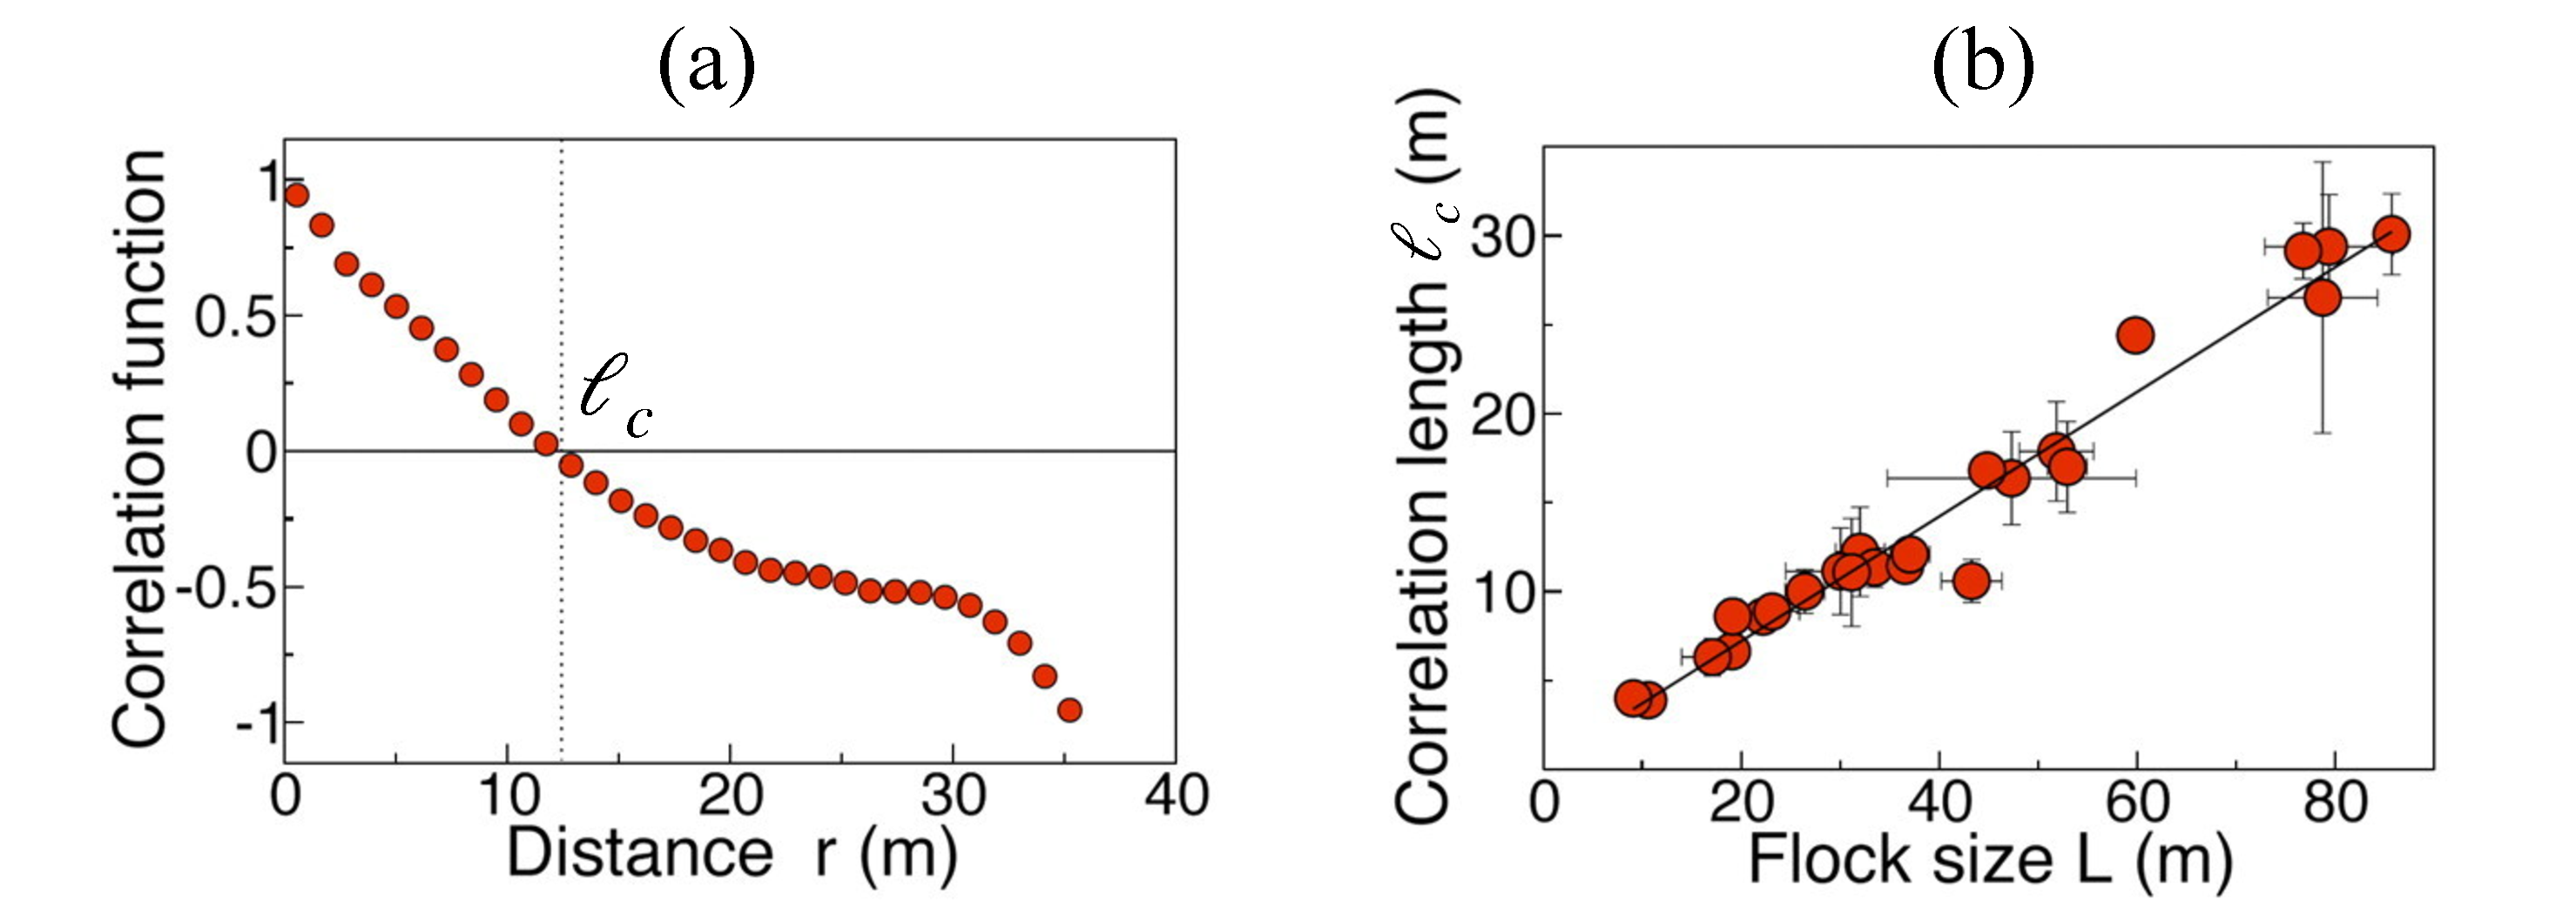
\includegraphics[width=.75\textwidth]{Figures/scalefree.pdf}
	\caption{(a) The correlation function $C(r)$ is the average inner product of the velocity fluctuations of pairs of birds at mutual distance $r$. This correlation function therefore measures to which extent the orientations of the velocity fluctuations are correlated. The function changes sign at $r=\ell_c$, which gives a good estimate of the average size of the correlated domains.(b) The orientation correlation length $\ell_c$ is plotted as a function of the linear size $L$ of the flock. Each point corresponds to a specific flocking event and it is an average over several instants of time in that event. The figure was reproduced from Ref.~\cite{cavagna2010scale}.
	}
	\label{scalefree}
	\end{center}
\end{figure}

Our purpose here will be to develop minimal models able to explain these features found not only in birds, but also in a variety of other systems.
Therefore, we will build our model from the example of birds for illustration purposes, but we won't consider the details of their ethology or morphology.
From far away, a flying bird is nothing but a polar object, meaning that is moves along a preferred direction set by its body axis.
Such feature is common in the systems we are interested in, so that in the following we will adopt an abstract representation
for which the bird is a simple arrow pointing along its direction of motion.

\paragraph*{Interactions with the environment}
Interactions between a biological systems and its environment are generally very complex and their quantitative description is here out of reach. 
Rather than solving the Navier-Stokes equations
to characterize the interaction of the bird with the surrounding air, 
we will here neglect inertia and the aerodynamics by assuming that the animal self-propels with a constant speed.
Such an approximation is arguably not so good for birds, but it turns out to be well verified for microscopic objects such as bacteria moving at low Reynolds numbers, or for any two dimensional active motion in the presence of a substrate.
Although setting the bird self propulsion speed to a constant leads to neglecting speed fluctuations, fluctuations in the direction of motion of the bird are generally still possible such that our model will retain orientational noise. 
 
 \paragraph*{Interactions with neighbors}
 Above, we have described the motion of a single bird, but below we will describe collective behaviors which implies to describe interactions between individuals.
 A prerequisite for flocking is that the birds seek to move together. 
 In the context of polar objects moving at constant speed, this effect is easily achieved via social rules leading to local alignment of velocities.
 Other types of interactions can of course be implemented. 
 For example, animals generally try to avoid colliding with each other, which can be described as a kind of short-ranged repulsion. Moreover, swarms or flocks usually show a certain degree of cohesion, which also suggests the presence of an effective attraction at long distances. 
 Another type of effective interactions may come from the medium our agents are moving into. An example of such interactions which we have studied in~\autoref{chap_phoretic} are phoretic interactions mediated by production/consumption and motility response to a chemical concentration. 
 Another prominent example are of course hydrodynamic interactions which play a central role in biological systems (cf~\autoref{chap_hydro}).
 Although these effects need to be considered when studying specific systems in details, they will enrich\footnote{Understand `complicate'.} the physics and may hide some of the universal features we are looking for. 
 In this lecture, we will thus restrict to the simplest setting where the agents of the model only interact via pairwise velocity alignment.


\section{The Vicsek model}

\subsection{Definition of the Vicsek class}

We now have all the necessary ingredients for a minimal model of collective motion.
The most famous one is arguably the Vicsek model~\cite{chate2020dry}, as it was first formulated by T. Vicsek and collaborators.
In the Vicsek setting, point-like particles move in two dimensions with constant speed $v_0$ and align their velocities with their neighbors in the presence of noise.
These rules mathematically translate in two dimensions into the following discrete time dynamics for the $i^{\rm th}$ particle's position $\bm r_i$ and velocity orientation $\theta_i$
\begin{subequations}
\label{eq_VM}
\begin{align}
\label{eq_VM_r}
\bm r_i^{t + \Delta t} & = \bm r_i^{t} + v_0 \Delta t \hat{\bm e}(\theta_i^{t + \Delta t}) \, , \\
\label{eq_VM_theta}
\theta_i^{t + \Delta t} & = {\rm Arg}\left[ \langle \hat{\bm e}(\theta_j^{t}) \rangle_{j \in \Omega_i} \right] + \eta \xi_i^t , 
\end{align}
\end{subequations} 
where $\hat{\bm e}(\theta) = (\cos(\theta),\sin(\theta))$ is the unit vector with orientation $\theta$, 
the average $\langle\cdot\rangle_{j \in \Omega_i}$ is done over the disk of radius $r_0$ centered in $i$: $\Omega_i \equiv \{ j ; \|\bm r_i  - \bm r_j\| \le r_0 \}$ 
(it therefore includes $i$ itself), and ${\rm Arg}[\bm v]$ returns the orientation of the vector $\bm v$.
The second term in the rhs of Eq.\eqref{eq_VM_theta} accounts for the angular fluctuations experienced by the particles, 
whose strength are set by the parameter $\eta$. 
$\xi_i^t$ is therefore a white noise with zero mean and unit variance:
$\langle \xi_i^t \xi_j^{t'} \rangle = \delta_{ij} \delta_{t t'}$ --hereafter angular brackets without indices are meant as averages over the noise.
In numerical simulations, the distribution of $\xi$ is usually taken uniform in $(-\pi;\pi]$ for simplicity, 
but other choices are possible (for instance Gaussian) and they do not qualitatively modify the dynamics 
so long as clockwise and counter-clockwise fluctuations remain equiprobable.
Similarly, different implementations of the Vicsek model have been proposed (e.g.\ considering continuous time dynamics, or with different forms of the noise etc...),
but those lead to large-scale collective features qualitatively similar to those of Eqs.~\eqref{eq_VM}.
For more details on the different numerical implementations of the Vicsek dynamics, see Ref.\cite{chate2020dry} and references therein.
Here, for practical purposes we'll consider the case where Eqs.~\eqref{eq_VM} are simulated in a square domain of linear size $L$ with periodic boundary conditions on all sides.

As for the Ising or $XY$ models for ferromagnets, the importance of the role of the Vicsek model in active matter studies stems from its simplicity and genericity.
Indeed, numerical and theoretical studies of the model allowed to uncover general physical principles which can be applied to a broad range of active matter systems.
In this context, Eqs.~\eqref{eq_VM} thus define a {\it Vicsek class} (or polar class), whose members all satisfy the following requirements:
\begin{itemize}
\item The alignment interactions between the particles are {\it local} and {\it polar}. 
Particles moreover do not point towards a preferred direction so that the dynamics is {\it isotropic}.  
\item {\it The particles are advected by their polarities.} 
While the polarity and velocity of Vicsek particles are identical, this constraint can be relaxed to some extent if the two remain coupled.
\item As a consequence of the previous point, the Vicsek class is inherently out of equilibrium. 
In particular, the dynamics does not conserve momemtum, so that it is not invariant by change of inertial frame and {\it Galilean symmetry is broken}.
\item The dynamics~\eqref{eq_VM} nevertheless {\it conserves the total particle number $N$} (there are no particle creation or annihilation).
\end{itemize}

\subsection{The phase diagram}

\label{sec_pd}

Rescaling space and time, we set $\Delta t$ and $r_0$ to unity. 
Therefore, the Vicsek model has three control parameters: $v_0$, $\eta$, and the mean particle density $\bar{\rho} \equiv N / L^2$.
Considering $v_0$ in a `reasonable' range --meaning not too small so that activity appears on scales accessible via simulations, 
or not too large so that the neighborhood of each particle is not completely randomized at each simulation step-- its specific value does not qualitatively affect the dynamics\footnote{Typically $v_0$ is taken between 0.1 and 1.}.
Hence, the dynamical behaviors of Vicsek particles can be explored tuning the remaining two parameters: the average particle density $\bar{\rho}$ and the strength of the noise $\eta$.

The phase diagram of the Vicsek model in the ($\bar{\rho}$,$\eta$) plane is shown in Fig.~\ref{figVM}(a). It includes three phases:
\begin{itemize}
\item At low particle densities and high noises, fluctuations dominate over alignment interactions and the system is thus globally disordered. 
Namely, the polarity and density correlations are exponential with a finite associated correlation length $\ell_c$. 
The system can thus be split into uncorrelated domains of linear size $> \ell_c$ so that from the law of large numbers the global polar order vanishes over large scales as
\begin{equation}
\Pi \equiv \langle \|\langle \hat{\bm e}(\theta_i^{t}) \rangle_{i=1\ldots N}\|\rangle_t \underset{L \gg \ell_c}{\sim} N^{-1/2} \sim L^{-1} .
\end{equation} 
\item At high densities and low noises, the mean number of neighbors of each particles is large enough so that the system forms 
a homogeneous ordered state in which particles move collectively along a randomly selected direction. 
This symmetry broken phase exhibits characteristic features such as scale free (power law) density and order correlations, 
as well as long-range orientational (polar) order.
Namely, as shown in Fig.~\ref{figVM}(c) the system's global polarization is found to decay with system size to a nonzero value $\Pi_\infty$, with power law finite-size corrections:
\begin{equation}
\label{eq_LRO}
\Pi \sim \Pi_{\infty} + A L^{-\omega} .
\end{equation} 
Here $\Pi_\infty$ and $A$ depend on the parameters $\bar{\rho}$ and $\eta$ and the details of the microscopic dynamics, 
while the exponent $\omega \simeq 2/3$~\cite{chate2020dry} is universal so that its value is the same throughout the homogeneous ordered phase and for all two dimensional systems in the Vicsek class (similarly to the critical exponents that we have used in~\autoref{chap_intro} to describe the transition to order in the Ising model).

Another peculiar feature of the ordered phase can be observed by measuring the statistics of the number of particle $n(t) \equiv \int_{\cal V}{\rm d}\bm r \, \sum_i \delta(\bm r - \bm r_i^t)$ into a sub-domain of volume $\cal V$.
Namely, measuring the mean and variance of $n$ in domains of increasing sizes one finds that
\begin{equation}
\langle \Delta n^2 \rangle \sim \langle n \rangle^\phi ,
\end{equation}
with $\phi \simeq 1.6$ (see Fig.~\ref{figVM}(c))~\cite{chate2020dry}. 
In a system with `normal' density fluctuations, the law of large number would impose that $\phi = 1$. 
Here, however, $\phi > 1$, i.e.\ the variance of $n$ grows faster than its mean, 
so that density fluctuations in the homogeneous ordered phase are deemed as `anomalous', or `giant'\footnote{Note that these giant density fluctuations are not related to any clustering phenomenon (e.g.\ like the motility induced phase separation discussed in~\autoref{chap_scalar}),
but instead due to the infinite correlation length of density fluctuations in an overall spatially homogeneous system.}.
\item Finally, contrary to magnetic systems at equilibrium (i.e.\ described by the Ising or $XY$ models) the transition to order in the Vicsek model does not occur via a second order transition but is best described as a phase separation scenario where elongated dense ordered liquid domains --which are usually referred to as \textit{bands}, see Fig.~\ref{figVM}(b)-- coexist with a dilute disordered gas.
Because of the coupling between density and order, these bands travel in the direction orthogonal to their axis.
They moreover have a well-defined width selected by the noise, so that their number grows with the mean particle density or system size,
and in large systems they arrange into a regular smectic configuration.
This {\it micro-phase separated} phase is thus distinct from the usual phase separation in which a single liquid domain occupies a macroscopic fraction of space and grows with density and system size.
\end{itemize}

%%%%%%%%%%%%%%%%%%%%%%%%%%%%
\begin{figure}[t!]
	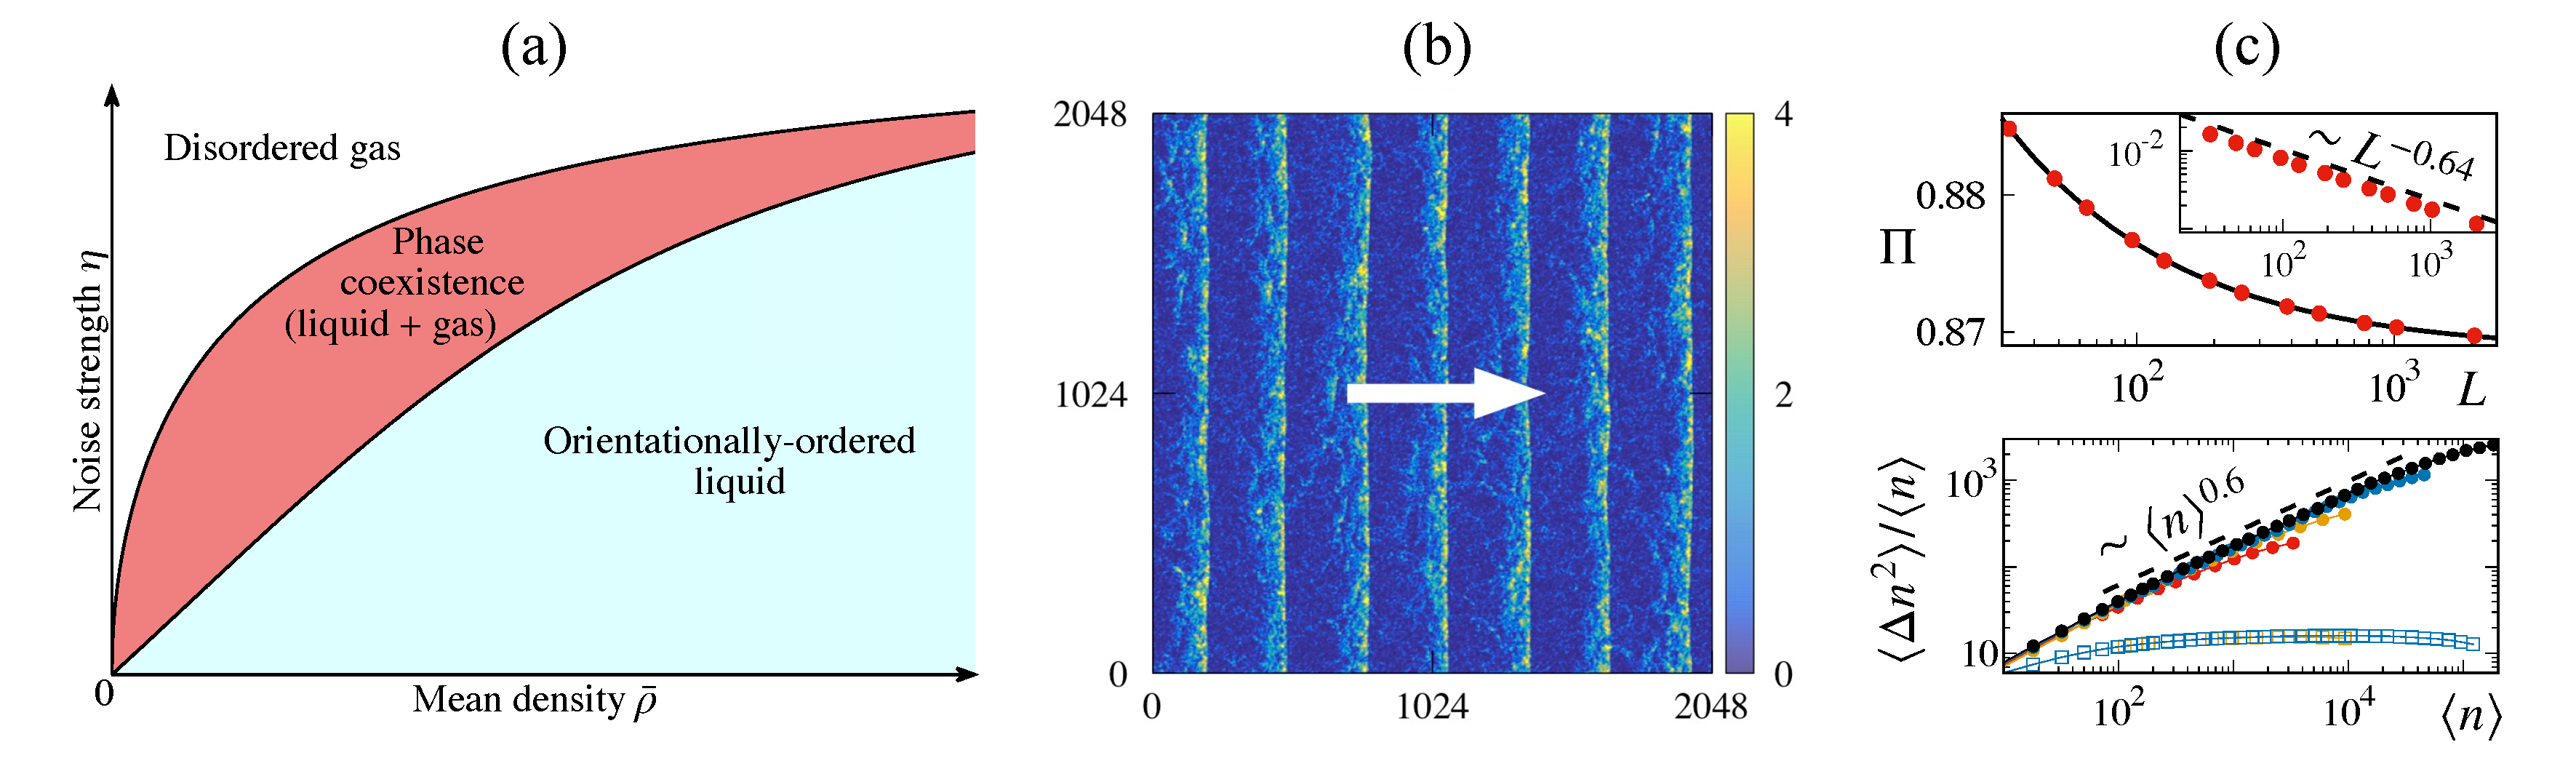
\includegraphics[width=\textwidth]{Figures/figVM.pdf}
	\caption{(a) The stylized phase diagram of the Vicsek model in the density-noise plane showing the three phases described in the text: disordered, homogeneously ordered, and the phase separated phase separating the two.
	(b) A snapshot of a regular smectic band configuration found in the phase-separated phase, the white arrow indicates the mean order direction and the color codes the local particle density. 
	Parameters are $\bar{\rho} = 1/2$, $\eta = 0.2$ and $v_0 = 0.5$.
	(c, top) Global polarization in the homogeneous ordered phase (in double-log representation) decreasing slower than a power law, the solid black line is a fit of the data by Eq.~\eqref{eq_LRO} giving $\Pi_\infty = 0.8685(2)$ and $\omega \simeq 0.64$. The inset shows the power law scaling of $\Pi - \Pi_\infty$ with system size.
	(c, bottom) $\langle \Delta n^2 \rangle/\langle n \rangle$ (see Sec.~\ref{sec_pd} for a definition) as a function of $\langle n \rangle$ showing anomalous density fluctuations in the ordered phase (filled circles) and normal fluctuations in the disordered phase (hollow squares). Different colors indicate different system sizes.
	Parameters for (c) are $\bar{\rho} = 2$, $v_0 = 0.5$, $\eta = 0.2$(ordered) and 0.6(disordered).
	All figures are reproduced from~\cite{DADAM_LesHouches}. 
	}
	\label{figVM}
\end{figure}
%%%%%%%%%%%%%%%%%%%%%%%%%%%%

\subsection{The hydrodynamic description of the Vicsek class}

It can be shown that a microscopic dynamics similar to that defined by Eqs.~\eqref{eq_VM} can be coarse-grained into hydrodynamic equations for the relevant physical fields which are the particle density $\rho$ and momentum $\bm w$ (or polarity):
\begin{align*}
\rho(\bm r,t) \equiv \left\langle \sum_i \delta(\bm r - \bm r_i^t) \right\rangle , \qquad 
\bm w(\bm r,t) = \rho(\bm r,t) \bm v(\bm r,t) \equiv \left\langle \sum_i \hat{\bm e}(\theta_i^t)\delta(\bm r - \bm r_i^t) \right\rangle .
\end{align*}
Using the Boltzmann-Ginzburg-Landau (BGL) approach detailed in Sec.~3 of Ref.~\cite{DADAM_LesHouches}, 
one can derive the set of partial differential equations governing the dynamics of $\rho$ and $\bm w$, known as the Toner Tu equations, which read
\begin{subequations}
\label{eq_TT}
\begin{align}
\label{eq_TT_rho}
& \partial_t \rho + \nabla \cdot \bm w = 0 , \\
\label{eq_TT_w}
& \partial_t \bm w + \lambda_1 (\bm w \cdot \nabla)\bm w + \lambda_2 (\nabla \cdot \bm w) \bm w + \lambda_3 \nabla |\bm w|^2 = 
-\frac{1}{2}\nabla \rho + \left( \mu(\rho) - \xi |\bm w|^2 \right) \bm w + \nu \Delta \bm w .
\end{align}
\end{subequations}
Thanks to the coarse-graining procedure, all coefficients of Eqs.~\eqref{eq_TT} can be expressed as functions of the microscopic dynamics parameters, i.e.\ density, noise and velocity.
This way it is possible to check from linear stability analysis and numerical simulations that Eqs.~\eqref{eq_TT} reproduce qualitatively the 
Vicsek model phase diagram of Fig.~\ref{figVM}(a) with the transition to collective motion occurring through a phase separated phase.
 
Although Eqs.~\eqref{eq_TT} were obtained starting from specific dynamical rules for the particles position and orientations, 
they contain almost all possible terms up to order 3 in fields and gradients that satisfy the constraints set by the Vicsek class,
so that their structure turns out to be quite generic and would not qualitatively change with the details of the dynamics.
In fact, Eqs.~\eqref{eq_TT} were first written by considering all relevant terms which satisfy the symmetries and conservation rules 
set by Eqs.~\eqref{eq_VM}:
\begin{itemize}
\item As a consequence of the particle number conservation, $\rho$ is a conserved field and Eq.~\eqref{eq_TT_rho} takes the form of a continuity equation with a mass flux $\bm w$, reflecting the fact that density is advected by order.
\item In Eq.~\eqref{eq_TT_w} the symmetry breaking associated with collective motion is accounted for by the Landau cubic term on the r.h.s. which, for $\mu(\bar{\rho}) > 0$, leads to the homogeneous ordered solution $\bm w = \sqrt{\mu(\bar{\rho}) / \xi} \hat{\bm e}_\|$ and $\hat{\bm e}_\|$ a unit vector pointing along an arbitrary direction.
\item The nonlinear terms on the l.h.s.\ of Eq.~\eqref{eq_TT_w} are moreover all allowed with arbitrary coefficients due to the absence 
of momentum conservation\footnote{In a compressible system, the advective term conserving momentum takes the form $\partial_t \bm w + \nabla \cdot (\bm w \bm w / \rho)$.}. 
Indeed, it is easy to check that they generally beak Galilean symmetry which would require the equations to be invariant under the transformation
\begin{equation*}
\bm w \to \bm w + \rho \bm u , \qquad \bm r \to \bm r - \bm u t ,
\end{equation*}
with $\bm u$ a constant velocity.
Moreover, because of these terms Eqs.~\eqref{eq_TT} generally cannot be written from minimizing of a free energy-type functional,
which highlights again the nonequilibrium nature of the underlying dynamics.
\end{itemize}
%Finally, we shall specify that the `simple' form of the pressure term ($\sim \nabla\rho$) in Eq.~\eqref{eq_TT_w} is a consequence of the point-wise nature of the particles, and considering short-range repulsion would lead to more a complicated expression. \\


In the remainder of these notes, we are going to focus on the derivation of large scale and long time universal properties of the fluctuating homogeneous ordered solution of Eqs.~\eqref{eq_TT}.
The approach presented below follows the seminal work by Toner and Tu~\cite{toner1995long,toner2012reanalysis}.
For readers interested in more details about the topic, we recommend the more recent treatment of Ref.~\cite{chate2024dynamic}.

\section{The transition to collective motion: linear stability analysis}

As Eqs.~\eqref{eq_TT} contain many terms which will not qualitatively affect the results derived below, 
for the sake of pedagogy we will study here simplified equations containing all relevant physical ingredients.
Namely, let us consider
\begin{subequations}
\label{eq_TT_new}
\begin{align}
\label{eq_TT_rho_new}
& \partial_t \rho + \nabla \cdot \bm w = 0 , \\
\label{eq_TT_w_new}
& \partial_t \bm w + \lambda (\bm w \cdot \nabla)\bm w = 
-\frac{1}{2}\nabla \rho + \left( \mu(\rho) - \xi |\bm w|^2 \right) \bm w + \nu \Delta \bm w ,
\end{align}
\end{subequations}
with now only one advection term in~\eqref{eq_TT_w_new}, but still with the coefficient $\lambda$ kept arbitrary.
Moreover, we will restrict most of the calculations to two dimensions.
For $\mu(\bar{\rho}) > 0$, the continuous theory admits the homogeneous ordered solution 
\begin{equation} \label{eq_hos}
\rho = \bar{\rho}, \qquad \bm w = \sqrt{\mu(\bar{\rho})/\xi} \hat{\bm e}_\| .
\end{equation}

In this section, we are interested in the stability of this solution.
We thus write the fields $\rho$ and $\bm w$ in terms of small perturbations around~\eqref{eq_hos}:
\begin{equation} 
\rho(\bm r,t) = \bar{\rho} + \delta\rho(\bm r,t), \qquad \bm w(\bm r,t) = \left( w_0 + \delta w_\|(\bm r,t) \right) \hat{\bm e}_\| + \delta w_\perp(\bm r,t) \hat{\bm e}_\perp ,
\end{equation}
with $w_0 \equiv \sqrt{\mu(\bar{\rho}) / \xi}$ and $\hat{\bm e}_\| \cdot \hat{\bm e}_\perp = 0$.
Keeping terms up to linear order, we obtain for the perturbations
\begin{subequations}
\label{eq_TT_lin}
\begin{align}
\label{eq_TT_lin_rho}
&\partial_t \delta \rho + \partial_\| \delta w_\| + \partial_\perp \delta w_\perp = 0, \\
\label{eq_TT_lin_para}
&\partial_t \delta w_\| + \lambda w_0  \partial_\| \delta w_\| = \left( \mu' w_0 - \frac{1}{2}\partial_\| \right)\delta \rho - 2\mu(\bar{\rho}) \delta w_\| + \nu \Delta \delta w_\| , \\
\label{eq_TT_lin_perp}
&\partial_t \delta w_\perp + \lambda w_0  \partial_\| \delta w_\perp =  - \frac{1}{2}\partial_\perp \delta \rho + \nu \Delta \delta w_\perp ,
\end{align}
\end{subequations}
where we have defined $\mu' \equiv {\rm d}\mu /{\rm d}\rho|_{\bar{\rho}}$ and $\partial_{\| , \perp} \equiv \hat{\bm e}_{\| , \perp} \cdot \nabla$.

Going into Fourier space, we recast Eqs.~\eqref{eq_TT_lin} into the linear system
\begin{equation*}
    \partial_t \begin{pmatrix}
        \delta\hat{\rho} \\
        \delta\hat{w}_\| \\
        \delta\hat{w}_\perp
    \end{pmatrix} = 
    \begin{pmatrix}
        0 & i q_\| & i q_\perp \\
        \mu'(\bar\rho)w_0 + \tfrac{1}{2}i q_\| & i\lambda w_0 q_\| - [2\mu(\bar\rho) + \nu q^2] & 0 \\
        \tfrac{1}{2}i q_\perp & 0 & i\lambda w_0 q_\| - \nu q^2
    \end{pmatrix}
    \begin{pmatrix}
        \delta\hat{\rho} \\
        \delta\hat{w}_\| \\
        \delta\hat{w}_\perp
    \end{pmatrix},
\end{equation*}
where $\delta\hat{\rho}(\bm q,t) = \int\dd\bm r \, \delta\rho(\bm r,t)\exp(i\bm q\cdot\bm r)$ and the other fields are defined in a similar way, while $\bm q = q_\|\hat{\bm e}_\| + q_\perp\hat{\bm e}_\perp$ with $q^2 = q_\|^2 + q_\perp^2$.
The stability of the homogeneous ordered solution is then set by the sign of the real part of the eigenvalue of the above matrix.

Given the configuration of the Vicsek bands (see~\autoref{figVM}), we moreover focus on perturbations in the direction longitudinal to the order here by setting $q_\perp = 0$.
This way, we directly obtain the eigenvalue associated to $\delta\hat{w}_\perp$: ${\cal Y}_\perp = -\nu q_\|^2 + i \lambda w_0 q_\|$,
whose real part is always negative.
The other two eigenvalues solve the second order polynomial equation
\begin{equation}\label{eq_poly_Y}
    {\cal Y}({\cal Y} + 2\mu(\bar\rho) + \nu q_\|^2 - i \lambda w_0 q_\|) - i q_\|\left(\mu'(\bar\rho) w_0 + \tfrac{1}{2}i q_\|\right) = 0.
\end{equation}
For $q_\| = 0$, it is straightforward to show that the solutions of this equation are ${\cal Y}_+ = 0$ and ${\cal Y}_- = -2\mu(\bar\rho)$.
As we are interested in long-wavelength instabilities, we focus here on ${\cal Y}_+$ and make use of the ansatz
\begin{equation*}
    {\rm Re}({\cal Y}) \underset{q_\| \to 0}{\simeq} q_\|^2, \qquad
    {\rm Im}({\cal Y}) \underset{q_\| \to 0}{\simeq} q_\|.
\end{equation*}
Replacing this ansatz in Eq.~\eqref{eq_poly_Y} we obtain at order $q_\|^2$
\begin{equation*}
    2 \mu(\bar\rho){\rm Re}({\cal Y}) - {\rm Im}^2({\cal Y}) + \lambda w_0 q_\| {\rm Im}({\cal Y}) + \tfrac{1}{2}q_\|^2 + i\left[ 2\mu(\bar\rho) {\rm Im}({\cal Y}) - q_\| \mu'(\bar\rho) w_0 \right] = 0,
\end{equation*}
from which we deduce
\begin{equation}
    {\rm Im}({\cal Y}) = \frac{\mu'(\bar\rho)w_0}{2\mu(\bar\rho)}q_\|, \qquad
    {\rm Re}({\cal Y}) = \frac{q_\|^2}{4\mu(\bar\rho)}\left[ \frac{(\mu'(\bar\rho))^2}{2 \mu(\bar\rho)\xi} - \frac{\lambda\mu'(\bar\rho)}{\xi} - 1 \right].
\end{equation}

\section{The Toner Tu theory: linearized hydrodynamics}

\subsection{Identification of the hydrodynamic modes}

Here, we consider a set of coefficients ($\lambda,\mu(\bar{\rho}),\xi,\nu$) so that we work deep enough in the ordered phase where~\eqref{eq_hos} is stable.
Comparing the r.h.s.\ of Eq.~\eqref{eq_TT_lin_para} with that of Eqs.~(\ref{eq_TT_lin_rho},\ref{eq_TT_lin_perp}), 
we find that $\delta w_\|$ is the only perturbation whose equation presents a damping term with coefficient $- 2\mu(\bar{\rho})$.
Consequently, longitudinal order perturbations typically relax on a finite timescale $\tau_\| \sim (2\mu(\bar{\rho}))^{-1}$,
while for density and transverse order perturbations are massless.
Therefore, $\delta w_\|$ can be considered as fast, 
while $\delta \rho$ and $\delta w_\perp$ are the hydrodynamic modes.

Using this separation of timescales between the fields, 
we neglect the time derivative in Eq.~\eqref{eq_TT_lin_para} and keep only the leading order terms in fields and gradients, which leads to
\begin{equation*}
\delta w_\| \simeq \frac{1}{2\mu(\bar{\rho})}\left( \mu' w_0 - \frac{1}{2}\partial_\| \right) \delta \rho .
\end{equation*}
Replacing this expression in Eq.~\eqref{eq_TT_lin_rho}, we finally get the closed set of equations
\begin{subequations}
\label{eq_TT_lin_closed}
\begin{align}
\label{eq_TT_lin_rho_closed}
&\partial_t \delta \rho + \tilde{v}_0\partial_\| \delta \rho + \partial_\perp \delta w_\perp = D_\rho \partial_\|^2 \delta\rho + \nabla \cdot \bm f_\rho, \\
\label{eq_TT_lin_perp_closed}
&\partial_t \delta w_\perp + \lambda w_0  \partial_\| \delta w_\perp =  - \frac{1}{2}\partial_\perp \delta \rho + \nu \Delta \delta w_\perp + f_\perp,
\end{align}
\end{subequations}
with $\tilde{v}_0 \equiv \mu' w_0 /  2\mu(\bar{\rho})$ and $D_\rho \equiv 1/4\mu(\bar{\rho})$.
As we are interested in calculating the response of the system to fluctuations, 
we have moreover included the noise terms $\bm f_\rho$ and $f_\perp$ in Eqs.~\eqref{eq_TT_lin_closed}.
We consider them as independent Gaussian white noises satisfying
\begin{equation} \label{eq_varf}
\langle f_{\rho,i}(\bm r,t)  f_{\rho,j}(\bm r',t') \rangle = \Delta_\rho \delta_{ij}\delta(\bm r - \bm r')\delta(t - t') , \qquad
\langle f_\perp(\bm r,t)f_\perp(\bm r',t') \rangle = \Delta_\perp \delta(\bm r - \bm r')\delta(t - t') .
\end{equation}
Note that the noise in Eq.~\eqref{eq_TT_lin_rho_closed} has to appear under a gradient term due to the particle number conservation constraint.

\subsection{Space-time correlations}

%\textcolor{blue}{I think that the FT has to be defined as $e^{-i(q \cdot r..)}$ to be consistent with the other formulas. I change it, in any case correct if it wrong. Also the term of the density noise misses an $i$.}

We now go to Fourier space:
\begin{equation*}
\delta \hat{\rho}(\bm q,\omega) = \int{\rm d}\bm r \int {\rm d}t \,  \delta\rho(\bm r,t)e^{i \bm q \cdot r - i \omega t} , \qquad
\delta \hat{w}_\perp(\bm q,\omega) = \int{\rm d}\bm r \int {\rm d}t \,  \delta w_\perp(\bm r,t)e^{i \bm q \cdot r - i \omega t},
\end{equation*}
where Eqs.~\eqref{eq_TT_lin_closed} are recast into the following linear system
\begin{equation}
\label{eq_TT_lin_fourier}
\begin{pmatrix}
\Gamma_\rho(\bm q,\omega) & -i q_\perp \\
-i\frac{q_\perp}{2} & \Gamma_\perp(\bm q,\omega) 
\end{pmatrix}
\begin{pmatrix}
\delta \hat{\rho}(\bm q,\omega) \\ \delta \hat{w}_\perp(\bm q,\omega)
\end{pmatrix}
=
\begin{pmatrix}
 -i\bm q \cdot \hat{ \bm f}_\rho(\bm q,\omega) \\ \hat{f}_\perp(\bm q,\omega)
\end{pmatrix} ,
\end{equation}
where $q_\|$ and $q_\perp$ are the wavenumbers associated respectively with the directions longitudinal and transverse to the global order, 
$\hat{ \bm f}_\rho$ and $\hat{f}_\perp$ are the Fourier transforms of the noises,
and we have defined 
\begin{equation*}
\Gamma_\rho(\bm q,\omega) \equiv i(\omega - \tilde{v}_0 q_\|) + D_\rho q_\|^2 , \qquad 
\Gamma_\perp(\bm q,\omega) \equiv i(\omega - \lambda w_0 q_\|) + \nu (q_\|^2 + q_\perp^2) .
\end{equation*}
In the following, we will focus on the scaling of the fields correlation functions in the large scale and long time limits, i.e.\ in the limits of vanishing $\omega$ and $q \equiv |\bm q|$.
In this regime the conserved noise term in Eq.~\eqref{eq_TT_lin_fourier} is subdominant w.r.t.\ $\hat{f}_\perp$, and we neglect it.
The system~\eqref{eq_TT_lin_fourier} is easily solved formally, and we find
\begin{equation}
\begin{pmatrix}
\delta \hat{\rho}(\bm q,\omega) \\ \delta \hat{w}_\perp(\bm q,\omega)
\end{pmatrix} = {\cal D}^{-1}(\bm q,\omega) 
\begin{pmatrix}
i q_\perp \\ \Gamma_\rho(\bm q,\omega)
\end{pmatrix} \hat{f}_\perp(\bm q,\omega) ,
\end{equation}
with ${\cal D}(\bm q,\omega) \equiv \Gamma_\rho(\bm q,\omega)\Gamma_\perp(\bm q,\omega) + q_\perp^2/2$.
In the limit where $\omega$ and $q$ go to zero, we simplify the expression of ${\cal D}(\bm q,\omega)$ by considering the following factorization
\begin{equation*}
{\cal D}(\bm q,\omega) \underset{\omega, q \to 0}{\simeq} -(\omega - \omega_+(\bm q))(\omega - \omega_-(\bm q)) ,
\end{equation*}
and where we assume that ${\rm Re}(\omega_\pm) \sim q$ and ${\rm Im}(\omega_\pm) \sim q^2$.
Replacing $w$ by $w_\pm(\bm q)$ in the expression of ${\cal D}(\bm q,\omega)$ and keeping terms up to order $q^2$ we end up with the dispersion relations 
$\omega_\pm(\bm q) = c_\pm(\theta_{\bm q}) q - i \varepsilon_\pm(\bm q)$, with
\begin{subequations}
\label{eq_speed_damp}
\begin{align}
\label{eq_speeds}
c_\pm(\theta_{\bm q}) &\equiv \frac{\lambda w_0 + \tilde{v}_0}{2}\cos(\theta_{\bm q}) \pm \sqrt{ \frac{(\lambda w_0 - \tilde{v}_0)^2}{4}\cos^2(\theta_{\bm q}) + \frac{\sin^2(\theta_{\bm q})}{2}} , \\
\label{eq_dampings}
\varepsilon_\pm(\bm q) &\equiv \frac{ [\tilde{v}_0\nu + D_\rho\lambda w_0\cos^2(\theta_{\bm q})  ]\cos(\theta_{\bm q}) - c_\pm(\theta_{\bm q})[\nu + D_\rho \cos(\theta_{\bm q}) ] }
{2 c_\pm(\theta_{\bm q}) + (\lambda w_0 + \tilde{v}_0)\cos(\theta_{\bm q}) } q^2 \sim q^2 ,
\end{align}
\end{subequations}
and where we have defined $\theta_{\bm q}$ as the angle between $\bm q$ and the global order ($q_\| = q\cos\theta_{\bm q}$ and $q_\perp = q\sin\theta_{\bm q}$). 
Using the expression of the noise variance in Fourier space $\langle \hat{f}_\perp(\bm q,\omega) \hat{f}_\perp(\bm q',\omega') \rangle = \Delta_\perp (2\pi)^3 \delta(\bm q + \bm q') \delta(\omega + \omega')$, we get the following expressions of the density and order correlation functions
\begin{subequations}
\label{eq_space_tim_cfs}
\begin{align}
\label{eq_space_tim_cfs_rho}
\left\langle \left|\delta \hat{\rho}(\bm q,\omega)\right|^2 \right\rangle &\underset{\omega, q \to 0}{\simeq} \frac{\Delta_\perp q_\perp^2}
{\left[ ( \omega - c_+(\theta_{\bm q}) q)^2  + \varepsilon^2_+(\bm q)   \right]\left[ ( \omega - c_-(\theta_{\bm q}) q)^2  + \varepsilon^2_-(\bm q)   \right]} , \\
\label{eq_space_tim_cfs_w}
\left\langle \left|\delta \hat{w}_\perp(\bm q,\omega)\right|^2 \right\rangle &\underset{\omega, q \to 0}{\simeq} \frac{\Delta_\perp (\omega - \tilde{v}_0 q_\|)^2}
{\left[ ( \omega - c_+(\theta_{\bm q}) q)^2  + \varepsilon^2_+(\bm q)   \right]\left[ ( \omega - c_-(\theta_{\bm q}) q)^2  + \varepsilon^2_-(\bm q)   \right]} .
\end{align}
\end{subequations}
As shown in Figs.~\ref{figmodes}(a,b), the density and order correlation functions plotted as function of $\omega$ at fixed $\bm q$ thus exhibit two peaks centred in $c_\pm(\theta_{\bm q})q$ and of widths $\varepsilon_\pm(\bm q)\sim q^2$.
Such structure reflects the presence of propagating density and order waves in the system with dispersion relations $\omega = \omega_\pm(\bm q)$.
Namely, these modes propagate with characteristic speeds $c_\pm(\theta_{\bm q})$ that depend on the orientation of $\bm q$ w.r.t.\ the mean order direction (see Fig.~\ref{figmodes}(c)). 
This is a direct consequence of fact that we are analyzing a symmetry broken phase.
Moreover, measuring the two different speeds of the modes in the direction longitudinal to order gives 
a direct indication of the absence of Galilean invariance in the system ($\tilde{v}_0 \ne \lambda w_0$).
The predicted life time of the modes takes a more conventional form set by $\varepsilon^{-1}_\pm(\bm q)\sim q^{-2} \sim \lambda^2$ with $\lambda$ the mode wavelength, which corresponds to the expected scaling for diffusive damping.

As we derived the structure of the propagating density and order modes from the generic hydrodynamic theory, 
we expect it to hold for a broad variety of systems.
Simulations of the Vicsek model~\eqref{eq_VM} indeed confirm the two-peaks structure predicted by Eqs.~\eqref{eq_space_tim_cfs}.
Measuring the peaks positions, one finds that they indeed scale linearly with $q$. 
The associated slope corresponds to the modes speeds which are found to vary with the orientation $\theta_{\bm q}$ 
in perfect agreement with Eq.~\eqref{eq_speeds} (as shown in Fig.~\ref{figmodes}(c)).
This phenomenology moreover holds beyond the Vicsek setting, as found in numerical simulations of a realistic model of self-propelled polar rods~\cite{Soni2020}
as well as in colloidal rollers experiments~\cite{geyer2018sounds}.

%%%%%%%%%%%%%%%%%%%%%%%%%%%%
\begin{figure}[t!]
	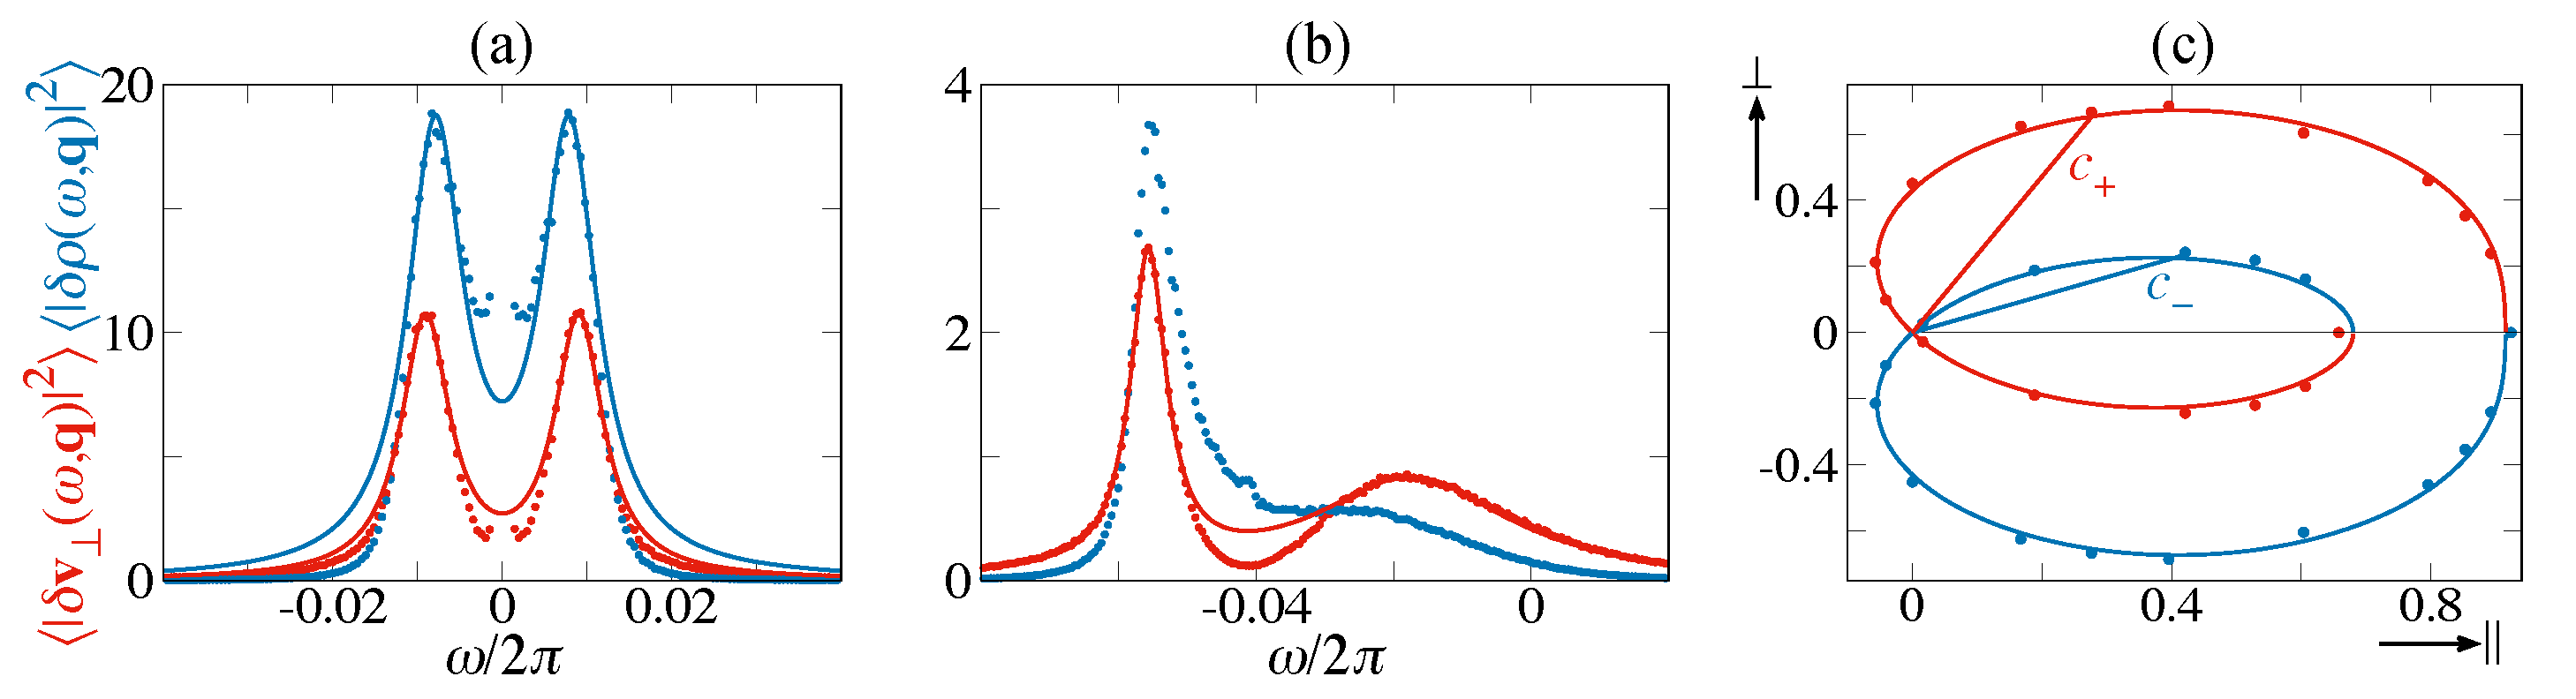
\includegraphics[width=\textwidth]{Figures/figmodes.pdf}
	\caption{(a,b) density(blue) and order(red) space time correlation functions as function of the frequency $\omega$ for $\theta_{\bm q} = \pi/2$(a) and $\pi/4$(b),
	respectively showing two symmetric and asymmetric peaks.
	When present, the continuous lines are fits of the numerical data (points) with Eqs.~\eqref{eq_space_tim_cfs}.
	(c) Polar representation of the mode speeds obtained from the scaling of the density and order correlation functions peaks position with $q$ at various values of $\theta_{\bm q}$. 
	The full line shows a fit of the data with Eq.~\eqref{eq_speeds}.}
	\label{figmodes}
\end{figure}
%%%%%%%%%%%%%%%%%%%%%%%%%%%%

\subsection{Equal-time correlation functions}

We now investigate on the nature of order as well as the presence of giant density fluctuations, which are both related to the equal-time correlation functions.
Equal-time density and order correlations are simply obtained by integrating Eqs.~\eqref{eq_space_tim_cfs} over the frequency $\omega$.
The full calculation can be carried out explicitly, but can be simplified considering the limit of small wavenumbers.
Indeed, although the two peaks in the space-time correlation functions are separated by $\sim q$, their respective widths $\sim q^2$ and their heights $\sim q^{-2}$.
Therefore, for $q \to 0$ the integral over $\omega$ of Eqs.~\eqref{eq_space_tim_cfs} will be dominated by the contributions from the individual peaks, 
which can be treated independently.
Using the relation $\int_{-\infty}^{+\infty} {\rm d}x \, [(x - x_0)^2 + \alpha^2]^{-1} = \pi/\alpha$, we thus get after little algebra
%\begin{subequations}
%\label{eq_eq_tim_cfs}
\begin{align*}
%\label{eq_eq_tim_cfs_rho}
\left\langle \left|\delta \hat{\rho}(\bm q)\right|^2 \right\rangle &\underset{q \to 0}{\simeq} \frac{\Delta_\perp \sin^2(\theta_{\bm q})}{ 2[c_+(\theta_{\bm q}) - c_-(\theta_{\bm q})]^2 }
\left( \frac{1}{\varepsilon_+(\bm q)} + \frac{1}{\varepsilon_-(\bm q)}  \right) , \\
%\label{eq_eq_tim_cfs_w}
\left\langle \left|\delta \hat{w}_\perp(\bm q)\right|^2 \right\rangle &\underset{q \to 0}{\simeq} \frac{\Delta_\perp}{ 2[c_+(\theta_{\bm q}) - c_-(\theta_{\bm q})]^2}
\left( \frac{ [ c_+(\theta_{\bm q}) - \tilde{v}_0\cos(\theta_{\bm q}) ]^2 }{\varepsilon_+(\bm q)} + \frac{[ c_-(\theta_{\bm q}) - \tilde{v}_0\cos(\theta_{\bm q}) ]^2}{\varepsilon_-(\bm q)}  \right) .
\end{align*}
%\end{subequations}
Using the expressions of the $c_\pm(\theta_{\bm q})$ and $\varepsilon_\pm(\bm q)$ given in Eq.~\eqref{eq_speed_damp} we finally rewrite these expressions into a more compact form:
\begin{equation}
\label{eq_eq_tim_cfs_simple}
\left\langle \left|\delta \hat{\rho}(\bm q)\right|^2 \right\rangle \underset{q \to 0}{\simeq} \frac{P_\rho(\theta_{\bm q})\sin^2(\theta_{\bm q})}{q^2} , \qquad
\left\langle \left|\delta \hat{w}_\perp(\bm q)\right|^2 \right\rangle \underset{q \to 0}{\simeq} \frac{P_\perp(\theta_{\bm q})}{q^2} ,
\end{equation}
with $P_\rho(\theta_{\bm q})$ and $P_\perp(\theta_{\bm q})$ two ${\cal O}(1)$ functions.
In agreement with numerical and experimental observations, density and order correlations are scale free (they scale like a power of $q$).
Moreover, although we derived Eqs.~\eqref{eq_eq_tim_cfs_simple} starting from a two dimensional theory, this result holds in arbitrary dimensions $d \ge 1$~\cite{toner2012reanalysis}.

\subsubsection{Giant density fluctuations}

The scaling of density fluctuations is obtained through the relation $\langle \Delta n^2 \rangle / \langle n \rangle \sim \lim_{q\to 0} \langle |\delta \hat{\rho}(\bm q)|^2 \rangle$.
Conventional density fluctuations are thus found when the Fourier space density correlation saturates to a constant value as $q \to 0$.
Here, on the contrary, $\langle |\delta \hat{\rho}(\bm q)|^2 \rangle$ diverges at vanishing wavenumbers like $q^{-2}$.
Using that $q \sim 1/L \sim 1/\langle n \rangle^{1/d}$, this implies
\begin{equation}
\langle \Delta n^2 \rangle \sim \langle n \rangle^\phi ,
\end{equation}
with $\phi = 1 + 2/d$.
Therefore, although our theory correctly predicts the existence of giant density fluctuations in all dimensions $d \ge 1$, 
the corresponding predicted exponent $\phi = 2$ for $d=2$ is larger than that measured in simulations or experiments (see e.g.\ Fig.~\ref{figVM}(c)).

\subsubsection{The nature of order}

For any dimension $d$, the typical strength of order fluctuations is set by 
\begin{equation}
\label{eq_order_flucts}
\left\langle \left|\delta {w}_\perp(\bm r)\right|^2 \right\rangle = \int \frac{{\rm d}\bm q}{(2\pi)^d} \left\langle \left|\delta \hat{w}_\perp(\bm q)\right|^2 \right\rangle 
\underset{q\to 0}{\sim} \int_{1/L}^{1/\Lambda} {\rm d}q \, q^{d-3} \underset{L\to +\infty}{\sim} 
\begin{cases}
L & (d=1) \\
\ln(L / \Lambda) & (d=2) \\
\Lambda^{2-d} & (d \ge 3)
\end{cases},
\end{equation}
with $\Lambda$ and ultra-violet cutoff length.
Eq.~\eqref{eq_order_flucts} predicts that the global polar order is destroyed by fluctuations in the limit of infinite system sizes for dimensions $d \le 2$.
More specifically, the logarithmic divergence predicted in $d=2$ is `slow enough' that, although the order vanishes asymptotically, the associated correlation length remains infinite.
Consequently, the global polarization decays with system size as $L^{-\kappa}$ with the exponent $0 < \kappa < 1$ usually nonuniversal.
This regime corresponds e.g.\ to that of the ordered phase of the two dimensional $XY$ model at equilibrium, and is named `quasi-long-range order'.
In $d \ge 3$, however, Eq.~\eqref{eq_order_flucts} predicts bounded polar order fluctuations so that order should remain long-ranged.\\
\\
In summary, we have derived the scaling of density and order correlation functions around the fluctuating homogeneous ordered solution of the Toner Tu equations~\eqref{eq_TT_new}.
The theory succeeds in predicting the presence of propagating density and order modes, giant density fluctuations, as well as the scale free correlations observed in numerical simulations and experiments.
However, some discrepancies persist: the exponent associated with giant density fluctuations is measured to be smaller than its predicted value, 
and most importantly the theory predicts a quasi-long-range order in two dimensions, 
at odds with observations of long-range orientational order~\eqref{eq_LRO} in numerical simulations of the two dimensional Vicsek model (see Fig.~\ref{figVM}(c)).
As we show below, these differences can be qualitatively explained by the fact that the effect of nonlinearities in the Toner Tu equations cannot be neglected in low dimensions, 
so that the linearized theory effectively breaks down.

\section{Some elements of the nonlinear Toner Tu theory}

To evaluate the importance of nonlinearities, we need to derive a nonlinear version of Eqs.~\eqref{eq_TT_lin_closed}.
Then, the question arises of which nonlinear terms should be kept and which should be discarded. The method to evaluate the relevance of these additional terms is called scaling analysis, or more formally the Renormalization Group (RG). 

The main idea behind this is the validity of the scaling hypothesis: when the system is largely correlated, i.e. $\ell_c \gg \Lambda$, the correlation length is the only relevant length scale of the dynamics, and it determines the macroscopic behavior through universal critical exponents. Indeed, all the microscopic details on scales smaller than $\ell_c$ do not really matter in a hydrodynamic description of the system. This is even more evident when $\ell_c \to \infty$, namely at the critical point of a phase transition or in the presence of spontaneous symmetry breaking with a Goldstone mode. In these cases, the system is scale invariant: the fluctuations extend on all the length scales (scale-free), and the physical properties are preserved when the observation scale is changed. To understand this, let's change the unit of space $r \to a r$, shrinking or dilating it with a scale factor $a$. We learned that when a system is scale-free, the correlation function of the order parameter decays with a power law $C(r) \sim r^{-\gamma}$. Performing the rescaling, we obtain
$$
C(ar) = \frac{1}{(ar)^{\gamma}} = a^{-\gamma} C(r) \ .
$$
The correlation function of the rescaled system is thus equal to the old correlation function multiplied by a constant factor: space rescaling does not change the physics when scale invariance is satisfied.  The RG is the set of transformations that allows to find the points of scale invariance (fixed points) of a specific field theory. It provides the information on how all the involved parameters have to change when space-time is rescaled, and the system is observed at larger and larger scales. 

We are now going to use RG arguments to understand which nonlinearities are relevant. For simplicity, we will consider here only the leading order nonlinearities, which are quadratic in the fields and linear in gradients. 
Carrying out the procedure detailed above, we find after enslaving the longitudinal order fluctuations\footnote{For the full derivation in the general case, see~\cite{toner2012reanalysis}.}
\begin{subequations}
\label{eq_TT_nlin_closed}
\begin{align}
\label{eq_TT_nlin_rho_closed}
&\partial_t \delta \rho + \tilde{v}_0\partial_\| \delta \rho + \partial_\perp \delta w_\perp + w_1 \partial_\perp( \delta \rho \delta w_\perp ) = 
D_\rho \partial_\|^2 \delta\rho + w_2\partial_\|  \delta \rho^2 + w_3 \partial_\|  \delta w_\perp^2 , \\
\label{eq_TT_nlin_perp_closed}
&\partial_t \delta w_\perp + \lambda w_0  \partial_\| \delta w_\perp + \lambda\delta w_\perp  \partial_\perp \delta w_\perp =  
- \frac{1}{2}\partial_\perp \delta \rho + \nu \Delta \delta w_\perp + g_1 \delta \rho \partial_\|  \delta w_\perp + g_2\delta w_\perp\partial_\|\delta \rho  + f_\perp,
\end{align}
\end{subequations}
and where, as previously, we have discarded the conserved noise term in Eq.~\eqref{eq_TT_nlin_rho_closed}.
Note, moreover, that all nonlinear terms in Eq.~\eqref{eq_TT_nlin_rho_closed} are total derivatives as a consequence of the particle number conservation.

We have shown from the linearized theory that the correlation functions of density and order in the ordered phase are scale free in $d\ge 2$,
therefore 
%from usual statistical mechanics arguments 
we assume the following scaling ansatz
\begin{equation} \label{eq_rescaling}
\bm r_\perp \to a \bm r_\perp , \quad r_\| \to a^\xi r_\| , \quad t \to a^z t , \quad \delta\rho \to a^{\chi_\rho}\delta\rho , \quad \delta w_\perp \to a^{\chi_\rho}\delta w_\perp ,
\end{equation}
with $a$ the given scaling factor.
The exponents $\xi$, $z$ $\chi_\rho$ and $\chi$ are {\it a priori} unknown, but as we will show below they can be fully determined for the linear theory.
$\xi$ measures the anisotropy of the scaling, while $\xi = 1$ corresponds to isotropy.
$z$ is called the dynamical exponent, and sets how the typical life time of perturbations scales with distances. 
$\chi_\rho$ and $\chi$ are the roughness exponents associated with density and order, respectively. 
They measure how the amplitude of fluctuations scales with distances. 

Applying the rescaling~\eqref{eq_rescaling} to Eqs.~\eqref{eq_TT_nlin_closed}, we get
\begin{subequations}
\label{eq_TT_rescalednonlin_closed}
\begin{align}
&\partial_t \delta \rho + \tilde{v}_0 a^{z-\xi} \partial_\| \delta \rho + a^{z + \chi - \chi_\rho -1} \partial_\perp \delta w_\perp + w_1 a^{z + \chi - 1} \partial_\perp( \delta \rho \delta w_\perp ) = \nonumber \\
& \qquad\qquad\qquad\qquad\qquad\qquad\qquad\qquad\qquad\qquad 
D_\rho a^{z-2\xi} \partial_\|^2 \delta\rho + w_2 a^{z + \chi_\rho - \xi}  \partial_\|  \delta \rho^2 + w_3 a^{z + 2\chi - \chi_\rho - \xi} \partial_\|  \delta w_\perp^2 , \\
&\partial_t \delta w_\perp + \lambda w_0 a^{z-\xi} \partial_\| \delta w_\perp + \lambda a^{z + \chi -1} \delta w_\perp  \partial_\perp \delta w_\perp  =  
- \frac{ a^{z + \chi_\rho - \chi - 1} }{2}\partial_\perp \delta \rho + \nu \left( a^{z-2\xi} \partial_\|^2 + a^{z-2} \partial_\perp^2 \right) \delta w_\perp \nonumber \\
& \qquad\qquad\qquad\qquad\qquad\qquad\qquad\qquad 
+ g_1 a^{z + \chi_\rho - \xi} \delta \rho \partial_\|  \delta w_\perp + g_2  a^{z + \chi_\rho - \xi} \delta w_\perp\partial_\|\delta \rho  + a^{\tfrac{z - 2\chi - (d-1) - \xi}{2}} f_\perp.
\end{align}
\end{subequations}
To calculate how the noise $f_\perp$ renormalizes upon the rescaling~\eqref{eq_rescaling}, we have used the relation~\eqref{eq_varf} 
as well as the fact that $\int {\rm d}\bm r' \, \delta(\bm r - \bm r') = 1$ and $ \int {\rm d}t' \, \delta(t - t') = 1$ must hold independently of $a$,
which implies $f_\perp^2 \to a ^{-(z + d-1 + \xi)} f_\perp^2$.
Each parameter of the theory could then be rescaled to preserve the same effective theory, for instance,
\begin{align*}
    D_\rho' &= D_\rho a^{z-2 \xi}, \\
    \nu' &= \nu a^{z-2}, \\
    \Delta_\perp' &= \Delta_\perp a^{(z-2\chi -(d-1)-\xi)/2}.
\end{align*}

To determine how the nonlinearities in Eqs.~\eqref{eq_TT_rescalednonlin_closed} renormalize upon the rescaling, 
we now evaluate the exponents in the linear theory. First, the continuity equation~\eqref{eq_TT_rho_new} combined with the dispersion relation $\omega \simeq c_\pm(\theta_{\bm q}) q$ implies that 
$c_\pm(\theta_{\bm q}) q \delta\hat{\rho} \sim q_\perp \delta \hat{w}_\perp$, which leads to $\chi_\rho = \chi$.
Secondly, the rescaling~\eqref{eq_rescaling} must leave the equal-time correlation functions~\eqref{eq_eq_tim_cfs_simple} invariant.
This can be achieved if the diffusion constants $\nu$ and $D_\rho$, as well as the noise $\Delta_\perp$, do not renormalize,
which from~\eqref{eq_TT_rescalednonlin_closed} implies the following hyperscaling relations
\begin{equation*}
z - 2 = 0, \qquad z - 2\xi = 0, \qquad z - 2\chi - (d-1) - \xi = 0 .
\end{equation*}
Solving for the three exponents, we then obtain their value given by the linear theory
\begin{equation}
z_{\rm lin} = 2, \qquad \xi_{\rm lin} = 1, \qquad \chi _{\rm lin} = 1 - \frac{d}{2} .
\end{equation}
In agreement with the results of the previous section, the linear theory thus predicts an isotropic scaling ($\xi = 1$), with diffusive damping of the modes ($z =2$)
and long-range order in $d \ge 3$ only ($\chi < 0$)\footnote{In two dimensions $\chi = 0$ but velocity correlations still diverge due to logarithmic corrections which cannot be captured by the scaling argument.}.

We now replace these values of the exponents in the nonlinear terms of  Eq.~\eqref{eq_TT_rescalednonlin_closed} to understand if the corresponding parameters grow or decrease upon rescaling. If they grow, the nonlinear terms are said to be {\it relevant} (positive scaling dimension), in the sense that they carry the system away from the linear fixed point. On the other hand, if they are irrelevant (negative scaling dimension) a small perturbation in their direction will be stable for the linear fixed point. We find that all nonlinearities renormalize as
\begin{equation}
\lambda; w_{1,2,3}; g_{1,2} \to a^{ \tfrac{4-d}{2} } \lambda; w_{1,2,3}; g_{1,2} .
\end{equation}
Therefore, for $d \ge 4$ all nonlinearities won't grow upon looking at the dynamics on larger scales. 
On the contrary, for $d < 4$ the strength of these nonlinearities grows as the theory is applied to larger scales and longer times, 
they are therefore relevant.
The upper critical dimension of the model, i.e.\ the dimension below which nonlinearities are important, is thus $d_c = 4$.

The the full nonlinear problem could be in principle addressed via renormalization group techniques, 
this is however a notoriously difficult task~\cite{toner2012reanalysis} which has not been performed so far.
Toner and Tu nevertheless managed to derive an expression for the scaling of the correlation functions using a matching procedure between the linear and nonlinear problems~\cite{toner1998flocks}.
They could show that the scaling of correlation functions could be obtained simply from their expressions~(\ref{eq_space_tim_cfs},\ref{eq_eq_tim_cfs_simple}) 
in the nonlinear theory with the renormalized noise variance and dampings
\begin{equation} \label{eq_renormalized_params}
\Delta_\perp(\bm q) = \Delta_\perp^0 q_\perp^{z - (d-1 + 2\chi + \xi)} {\cal F}_\Delta \left( \frac{q_\| }{q_\perp^\xi} \right) , \qquad
\varepsilon_\pm(\bm q) = \varepsilon_\pm^0 q_\perp^z {\cal F}_\pm \left( \frac{q_\| }{q_\perp^\xi} \right) ,
\end{equation}
while the modes speeds $c_\pm(\theta_{\bm q})$ remain those given by the linear theory, 
and where the functions ${\cal F}_\perp$ and ${\cal F}_\pm$ are unknown but universal and satisfy
\begin{equation*}
{\cal F}_\Delta(x) \underset{x \to 0}{\to} {\rm const} , \qquad {\cal F}_\Delta(x) \underset{x \to +\infty}{\to} x^{\tfrac{z - (d-1 + 2\chi + \xi)}{\xi}} ,\qquad
{\cal F}_\pm(x) \underset{x \to 0}{\to} {\rm const} , \qquad {\cal F}_\pm(x) \underset{x \to +\infty}{\to} x^{\tfrac{z}{\xi}} .
\end{equation*}
Replacing Eq.~\eqref{eq_renormalized_params} into Eq.~\eqref{eq_eq_tim_cfs_simple}, for instance, leads up to some ${\cal O}(1)$ factors
to the following expression of the equal-time correlation functions
\begin{equation} \label{eq_nl_scaling}
\left\langle \left|\delta \hat{\rho}(\bm q)\right|^2 \right\rangle \underset{q \to 0}{\simeq} \frac{q_\perp^{2 - (d-1 + 2\chi + \xi)}}{q^2}{\cal F}_\rho \left( \frac{q_\| }{q_\perp^\xi} \right)  , \qquad
\left\langle \left|\delta \hat{w}_\perp(\bm q)\right|^2 \right\rangle \underset{q \to 0}{\simeq} q_\perp^{- (d-1 + 2\chi + \xi)}{\cal F}_\perp \left( \frac{q_\| }{q_\perp^\xi} \right) ,
\end{equation}
with ${\cal F}_{\rho,\perp}(x) \underset{x \to 0}{\to} {\rm const}$ and  ${\cal F}_{\rho,\perp}(x) \underset{x \to 0}{\to} x^{\tfrac{- (d-1 + 2\chi + \xi)}{\xi}}$.
The scaling form~\eqref{eq_nl_scaling} was later confirmed by numerical simulations of the Vicsek model (for the full analysis, see~\cite{mahault2019TT}),
with the numerically determined exponents in two dimensions
\begin{equation} \label{eq_exps}
\chi = -0.31(2) , \qquad \xi = 0.95 (2) , \qquad  z = 1.33(2) .
\end{equation}
Therefore, it turns out that the scaling of correlation functions is nearly isotropic ($\xi \lesssim 1$), 
while the true long range order is confirmed ($\chi < 0$)\footnote{Actually, the exponent $\omega$ defined in Sec.~\ref{sec_pd} can be shown to be equal to $-2\chi$.}.
The fact that $z< 2$ moreover indicates that density and order fluctuations are damped 
on large scales more heavily than predicted by the linear theory (their life time scales as $\lambda^z$, with $\lambda$ their wavelength).
Going back to the giant density fluctuations, the exponents~\eqref{eq_exps} moreover imply that $\phi \simeq 1.67$, 
which is a value compatible with that usually directly measured from the scaling of $\langle \Delta n^2\rangle$ with $\langle n \rangle$ (see Fig.~\ref{figVM}(c)).

Although no proper RG treatment of Eqs.~\eqref{eq_TT_nlin_closed} has been carried out yet, recently alternative approaches based on scaling arguments have been proposed to predict the values of the exponents in dimension $d=2$.
Namely, the idea is first to note that for $\delta w_\perp$ to be a Goldstone mode, the deterministic part of its dynamics must be written as a total derivative (otherwise, the nonlinear terms that are not total derivatives effectively generate a mass), which implies in practice that $g_1 = g_2$.
As a consequence, the noise in Eq.~\eqref{eq_TT_nlin_perp_closed} cannot be renormalized by nonlinearities as the short scales of the theory are integrated out, since it is the only contribution on the r.h.s.\ that is not a total derivative. 
Hence, at the RG fixed point the hyperscaling relation
\begin{equation*}
    z = 1 + 2\chi + \xi,
\end{equation*}
must be satisfied.
Two other scaling relations can moreover be obtained by noting that Eqs.~\eqref{eq_TT_nlin_closed} remain invariant under a generalized Galilean transformation.
The details of this argument are quite subtle, so we refer to~\cite{chate2024dynamic} for details, but as a result the coefficients $w_{1,2,3},\lambda,g_1$ in front of the nonlinearities in Eqs.~\eqref{eq_TT_nlin_closed} are also not renormalized under RG transformation.
This implies two other scaling relations at the fixed point:
\begin{equation*}
    \chi + z - 1 = 0, \qquad
    \chi + z - \xi = 0.
\end{equation*}
Solving for $\chi$, $\xi$ and $z$, we then conclude that
\begin{equation}
    \chi = -\frac{1}{3}, \qquad
    \xi = 1, \qquad
    z = \frac{4}{3}.
\end{equation}
Note that these values are indeed very close to the ones obtained from numerical simulations (Eq.~\eqref{eq_exps}).

 % Appart from the giant density fluctuations, the scaling laws giving access to the values of the exponents $\chi$, $\xi$ and $z$ are difficult to measure
 % due to the strong finite size effects present in the Vicsek model. 
 % These effects are moreover amplified considering more realistic models with repulsion, or in experiments.
 % Therefore, for far there has not been any convincing experimental confirmation of the values of the exponents~\eqref{eq_exps}.
